\documentclass{beamer}\usepackage[]{graphicx}\usepackage[]{color}
%% maxwidth is the original width if it is less than linewidth
%% otherwise use linewidth (to make sure the graphics do not exceed the margin)
\makeatletter
\def\maxwidth{ %
  \ifdim\Gin@nat@width>\linewidth
    \linewidth
  \else
    \Gin@nat@width
  \fi
}
\makeatother

\definecolor{fgcolor}{rgb}{0.345, 0.345, 0.345}
\newcommand{\hlnum}[1]{\textcolor[rgb]{0.686,0.059,0.569}{#1}}%
\newcommand{\hlstr}[1]{\textcolor[rgb]{0.192,0.494,0.8}{#1}}%
\newcommand{\hlcom}[1]{\textcolor[rgb]{0.678,0.584,0.686}{\textit{#1}}}%
\newcommand{\hlopt}[1]{\textcolor[rgb]{0,0,0}{#1}}%
\newcommand{\hlstd}[1]{\textcolor[rgb]{0.345,0.345,0.345}{#1}}%
\newcommand{\hlkwa}[1]{\textcolor[rgb]{0.161,0.373,0.58}{\textbf{#1}}}%
\newcommand{\hlkwb}[1]{\textcolor[rgb]{0.69,0.353,0.396}{#1}}%
\newcommand{\hlkwc}[1]{\textcolor[rgb]{0.333,0.667,0.333}{#1}}%
\newcommand{\hlkwd}[1]{\textcolor[rgb]{0.737,0.353,0.396}{\textbf{#1}}}%

\usepackage{framed}
\makeatletter
\newenvironment{kframe}{%
 \def\at@end@of@kframe{}%
 \ifinner\ifhmode%
  \def\at@end@of@kframe{\end{minipage}}%
  \begin{minipage}{\columnwidth}%
 \fi\fi%
 \def\FrameCommand##1{\hskip\@totalleftmargin \hskip-\fboxsep
 \colorbox{shadecolor}{##1}\hskip-\fboxsep
     % There is no \\@totalrightmargin, so:
     \hskip-\linewidth \hskip-\@totalleftmargin \hskip\columnwidth}%
 \MakeFramed {\advance\hsize-\width
   \@totalleftmargin\z@ \linewidth\hsize
   \@setminipage}}%
 {\par\unskip\endMakeFramed%
 \at@end@of@kframe}
\makeatother

\definecolor{shadecolor}{rgb}{.97, .97, .97}
\definecolor{messagecolor}{rgb}{0, 0, 0}
\definecolor{warningcolor}{rgb}{1, 0, 1}
\definecolor{errorcolor}{rgb}{1, 0, 0}
\newenvironment{knitrout}{}{} % an empty environment to be redefined in TeX

\usepackage{alltt}
\usepackage{xcolor}
\usepackage{natbib}
\usepackage{multicol}
\usepackage{booktabs}
\usepackage{wasysym}
\usepackage{graphicx}
\usepackage{color}
\usepackage{lmodern}
\usepackage{array}
\usepackage{amsmath}
\usepackage{dcolumn}

\usetheme{Frankfurt}
%\usecolortheme{beaver}
\setbeamertemplate{footline}
{
  \leavevmode%
  \hbox{%
  \begin{beamercolorbox}[wd=.3\paperwidth,ht=2.25ex,dp=1ex,center]{author in head/foot}%
    \usebeamerfont{author in head/foot}\insertshortauthor \hspace{1em} %(\insertshortinstitute)
  \end{beamercolorbox}%
  \begin{beamercolorbox}[wd=.4\paperwidth,ht=2.25ex,dp=1ex,center]{title in head/foot}%
    \usebeamerfont{title in head/foot}\insertshorttitle
  \end{beamercolorbox}%
  \begin{beamercolorbox}[wd=.3\paperwidth,ht=2.25ex,dp=1ex,right]{author in head/foot}%
    \usebeamerfont{author in head/foot}\insertdate \hspace{2em}
    \insertframenumber{} / \inserttotalframenumber\hspace*{1em}
  \end{beamercolorbox}}%
  \vskip0pt%
}
\definecolor{beamer@sbred}{rgb}{0.65,0.15,0.18}
\setbeamercolor{title}{fg=beamer@sbred,bg=black!5}
\setbeamercolor{structure}{fg=beamer@sbred}
\setbeamercolor{frametitle}{fg=beamer@sbred}
\setbeamercolor{palette primary}{fg=beamer@sbred,bg=black!10}
\setbeamercolor{palette secondary}{fg=beamer@sbred}
\setbeamercolor{palette tertiary}{bg=beamer@sbred}
\setbeamercolor{palette quaternary}{fg=white,bg=beamer@sbred}
\setbeamertemplate{itemize items}[default]
\setbeamertemplate{enumerate items}[default]
\setbeamersize{text margin left=1em,text margin right=1em}
\DeclareTextFontCommand{\emph}{\color{beamer@sbred}}

\author[Kraft, Weber, Lebo]{Patrick Kraft \and
Christopher Weber \and
Matthew Lebo}
\institute{Stony Brook University \and
University of Arizona}
 \title{R Package ArfimaMLM}
 \subtitle{An Effective Approach to the Repeated Cross-Sectional Design}
 \date{\today}
\IfFileExists{upquote.sty}{\usepackage{upquote}}{}
\begin{document}
\frame{\titlepage}

\section{Overview}
\subsection{}
\begin{frame}%[allowframbreaks]
\frametitle{Introduction}
\begin{itemize}
\item Implementation of \emph{ArfimaMLM} approach presented by Lebo and Weber (``An Effective Approach to the Repeated Cross-Sectional Design'', \textit{AJPS} \citeyear{lebo2015effective}) in \texttt{R}.
\item \emph{Basic idea}: Correcting for temporal autocorrelation in repeated cross-sectional data (as well as panel data).
\item \emph{Key Aspects}:
\begin{itemize}
\item Individual observations are embedded within multiple, sequential time-points.
\item Retrieve estimates at the individual-level and at the aggregate level.
\item Allows use of variables that vary only within cross-sections and some that vary between cross-sections (e.g., unemployment rate)
\item Box-Jenkins and fractional differencing techniques can control for autocorrelation at level-2. \citep[e.g.][]{box1996dynamics,lebo2000you,clarke2003fractional}
\item Introduce double filtering to clean up two kinds of autocorrelation.
\end{itemize}
\end{itemize}
\end{frame}

\subsection{}
\begin{frame}[fragile]\scriptsize%[allowframbreaks]
\frametitle{Description of Package}
\begin{knitrout}
\definecolor{shadecolor}{rgb}{0.969, 0.969, 0.969}\color{fgcolor}\begin{kframe}
\begin{alltt}
\hlkwd{arfimaMLM}\hlstd{(formula, data, timevar}
          \hlstd{,} \hlkwc{d} \hlstd{=} \hlstr{"Hurst"}\hlstd{,} \hlkwc{arma} \hlstd{=} \hlkwa{NULL}
          \hlstd{,} \hlkwc{ecmformula} \hlstd{=} \hlkwa{NULL}\hlstd{,} \hlkwc{decm} \hlstd{=} \hlstr{"Hurst"}
          \hlstd{,} \hlkwc{drop} \hlstd{=} \hlnum{5}\hlstd{,} \hlkwc{report.data} \hlstd{=} \hlnum{TRUE}\hlstd{, ...)}

\hlkwd{arfimaMLM}\hlstd{(y.ydif} \hlopt{~} \hlstd{x1.xdif} \hlopt{+} \hlstd{x1.fd} \hlopt{+} \hlstd{x2} \hlopt{+} \hlstd{z1.fd} \hlopt{+} \hlstd{z2.fd}
          \hlopt{+} \hlstd{(}\hlnum{1} \hlopt{|} \hlstd{time)}
          \hlstd{,} \hlkwc{data} \hlstd{= data,} \hlkwc{timevar} \hlstd{=} \hlstr{"time"}\hlstd{, ...)}

\hlkwd{arfimaMLM}\hlstd{(y.ydif} \hlopt{~} \hlstd{x1.xdif} \hlopt{+} \hlstd{x1.fd} \hlopt{+} \hlstd{x2} \hlopt{+} \hlstd{z1.fd} \hlopt{+} \hlstd{z2.fd} \hlopt{+} \hlstd{ecm}
          \hlopt{+} \hlstd{(}\hlnum{1} \hlopt{|} \hlstd{time)}
          \hlstd{,} \hlkwc{data} \hlstd{= data,} \hlkwc{timevar} \hlstd{=} \hlstr{"time"}
          \hlstd{,} \hlkwc{d} \hlstd{=} \hlstr{"Sperio"}
          \hlstd{,} \hlkwc{ecmformula} \hlstd{= y.mean} \hlopt{~} \hlstd{x1.mean}
          \hlstd{,} \hlkwc{decm} \hlstd{=} \hlstr{"ML"}\hlstd{, ...)}

\hlkwd{arfimaMLM}\hlstd{(y.ydif} \hlopt{~} \hlstd{x1.xdif} \hlopt{+} \hlstd{x1.fd} \hlopt{+} \hlstd{x2} \hlopt{+} \hlstd{z1.fd} \hlopt{+} \hlstd{z2.fd} \hlopt{+} \hlstd{ecm}
          \hlopt{+} \hlstd{(}\hlnum{1} \hlopt{+} \hlstd{x1.dif} \hlopt{|} \hlstd{time)}
          \hlstd{,} \hlkwc{data} \hlstd{= data,} \hlkwc{timevar} \hlstd{=} \hlstr{"time"}
          \hlstd{,} \hlkwc{d} \hlstd{=} \hlkwd{list}\hlstd{(}\hlkwc{y} \hlstd{=} \hlstr{"Hurst"}\hlstd{,} \hlkwc{x1} \hlstd{=} \hlstr{"GPH"}\hlstd{,} \hlkwc{z1} \hlstd{=} \hlstr{"Sperio"}\hlstd{,} \hlkwc{z2} \hlstd{=} \hlnum{0.25}\hlstd{)}
          \hlstd{,} \hlkwc{arma} \hlstd{=} \hlkwd{list}\hlstd{(}\hlkwc{y} \hlstd{=} \hlkwd{c}\hlstd{(}\hlnum{1}\hlstd{,}\hlnum{0}\hlstd{),} \hlkwc{z2} \hlstd{=} \hlkwd{c}\hlstd{(}\hlnum{0}\hlstd{,}\hlnum{1}\hlstd{)), ...)}
\end{alltt}
\end{kframe}
\end{knitrout}
\end{frame}

\section{Simulational Scenario}
\subsection{}
\begin{frame}%[allowframbreaks]
\frametitle{Simulational Scenario}


\begin{itemize}
\item \emph{Scenario}: repeated cross-sectional dataset with 100 timepoints and 500 units within each timepoint
\item \emph{Independent variables:}
\begin{itemize}
\item $x_1 \sim \mathcal{N}(\mu=\bar{X}_{1t},\sigma^2=2)$; $\bar{X}_{1t}$ follows a fractionally integrated series with $d=0.3$ and a mean of 5
\item $x_2 \sim \mathcal{N}(\mu=0,\sigma^2=40)$
\item $z_1 \sim \mathcal{N}(\mu=\bar{Z}_{1t},\sigma^2=3)$; $\bar{Z}_{1t}$ follows a fractionally integrated series with $d=0.1$ and a mean of 2
\item $Z_{2t}$ follows a fractionally integrated series with $d=0.25$ and a mean of 3 ($Z_{2t}$ does not differ within timepoints)
\end{itemize}
\item \emph{Dependent Variable}:
\begin{align*}
y &=\bar{Y}_t+\beta_{1t} * x_1 - 0.05 * x_2 + 0.3 * \bar{Z}_{1t} + 0 * Z_{2t} + \epsilon &\text{ , where} \nonumber \\
\beta_{1t} &\sim \mathcal{N}(\mu=0.2,\sigma^2=0.1) & \nonumber \\
\epsilon &\sim \mathcal{N}(\mu=0,\sigma^2=1), &
\end{align*}
\footnotesize{where $\bar{Y}_t$ follows a fractionally integrated series with $d=0.4$ and a mean of 10}
\end{itemize}
\end{frame}

\subsection{}
\begin{frame}[fragile]%[allowframbreaks]
\frametitle{Data Overview I}
\begin{knitrout}
\definecolor{shadecolor}{rgb}{0.969, 0.969, 0.969}\color{fgcolor}\begin{kframe}
\begin{alltt}
\hlstd{data[}\hlnum{496}\hlopt{:}\hlnum{505}\hlstd{,]}
\end{alltt}
\begin{verbatim}
    time       x1         x2          z1       z2         y
496    1 2.782894  99.649591  4.52390786 2.222936  6.556912
497    1 4.666993  15.769259  4.58101935 2.222936 10.326180
498    1 3.479995 -23.151975 -0.05688266 2.222936 13.371325
499    1 4.927197  -3.963808  6.34666239 2.222936 12.706198
500    1 4.671967  33.751661  0.60743779 2.222936  9.181135
501    2 2.888744  26.234304  2.96382521 1.969999 10.004992
502    2 3.334345 -22.937614  3.75093669 1.969999 13.311789
503    2 5.516160   5.706410  6.43928311 1.969999 11.906759
504    2 8.195076  31.802270  4.88271529 1.969999 14.047000
505    2 7.086206  95.629309  2.69268251 1.969999  6.587762
\end{verbatim}
\end{kframe}
\end{knitrout}
\end{frame}

\subsection{}
\begin{frame}%[allowframbreaks]
\frametitle{Data Overview II}
\begin{figure}[ht]\centering
\caption{Plot of Dependent Variable y Across Time}
\begin{knitrout}
\definecolor{shadecolor}{rgb}{0.969, 0.969, 0.969}\color{fgcolor}
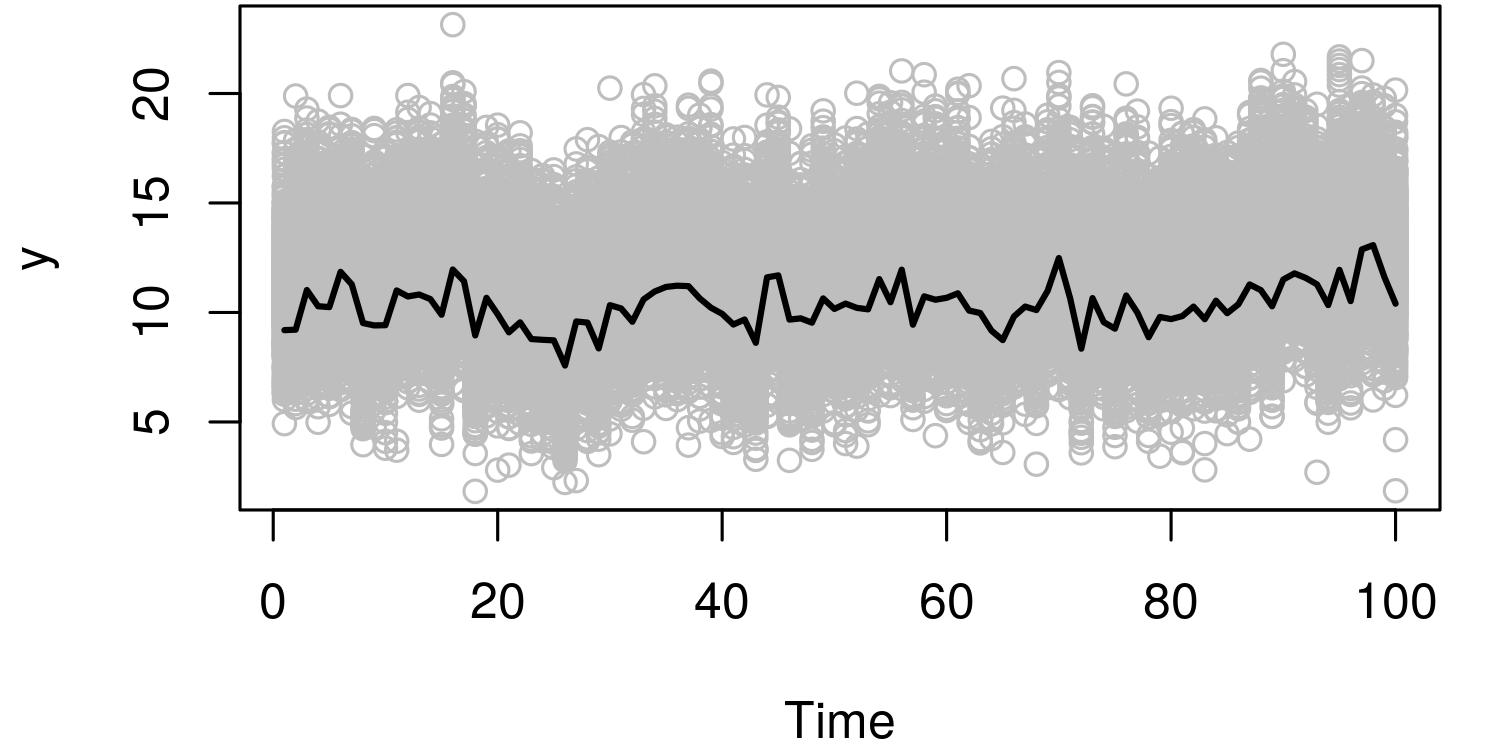
\includegraphics[width=\maxwidth]{figure/d-1} 

\end{knitrout}
\end{figure}
\end{frame}

\subsection{}
\begin{frame}%[allowframbreaks]
\frametitle{Data Overview III}
\begin{figure}[ht]\centering
\caption{Plot of Independent Variables Across Time}
\begin{knitrout}
\definecolor{shadecolor}{rgb}{0.969, 0.969, 0.969}\color{fgcolor}
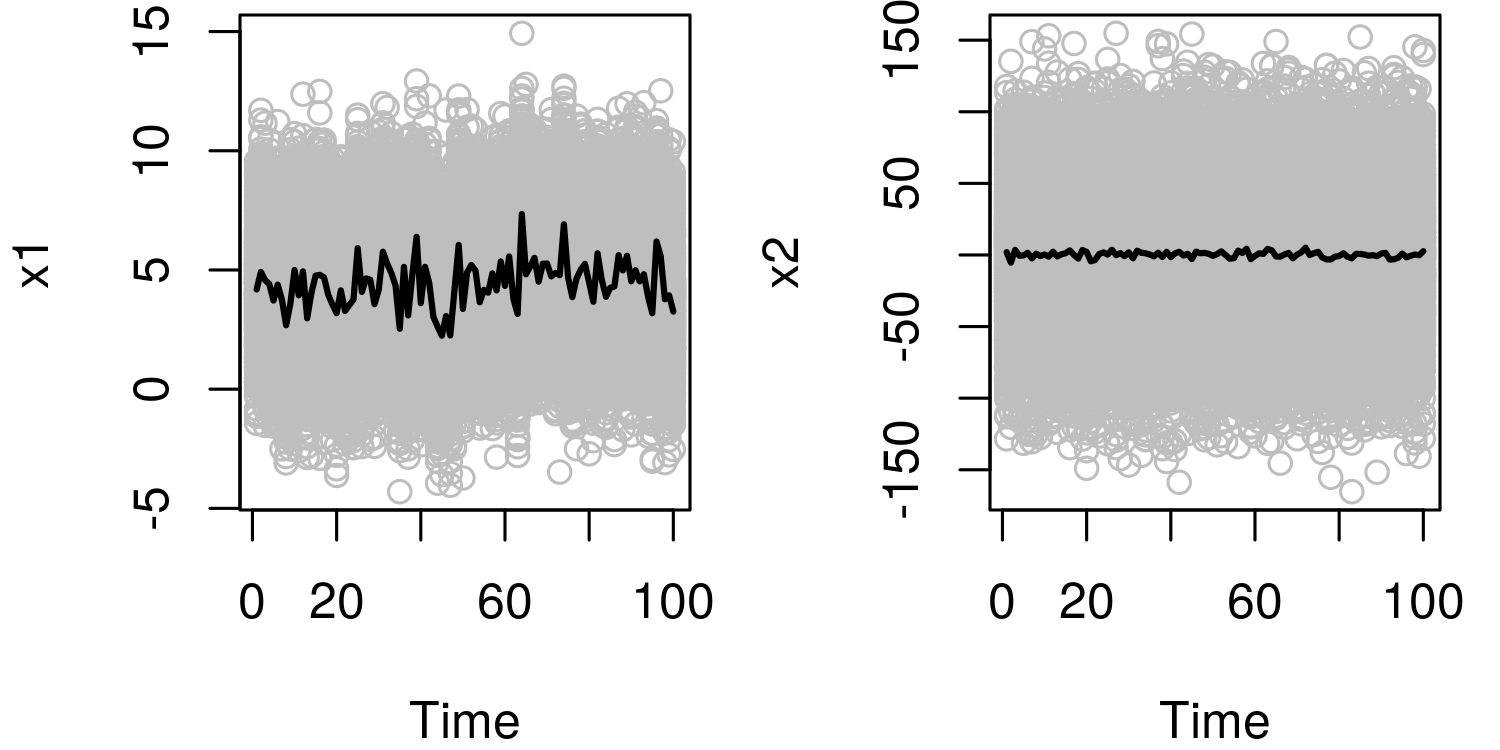
\includegraphics[width=\maxwidth]{figure/e-1} 

\end{knitrout}
\end{figure}
\end{frame}

\subsection{}
\begin{frame}%[allowframbreaks]
\frametitle{Data Overview IV}
\begin{figure}[ht]\centering
\caption{Plot of Independent Variables Across Time}
\begin{knitrout}
\definecolor{shadecolor}{rgb}{0.969, 0.969, 0.969}\color{fgcolor}
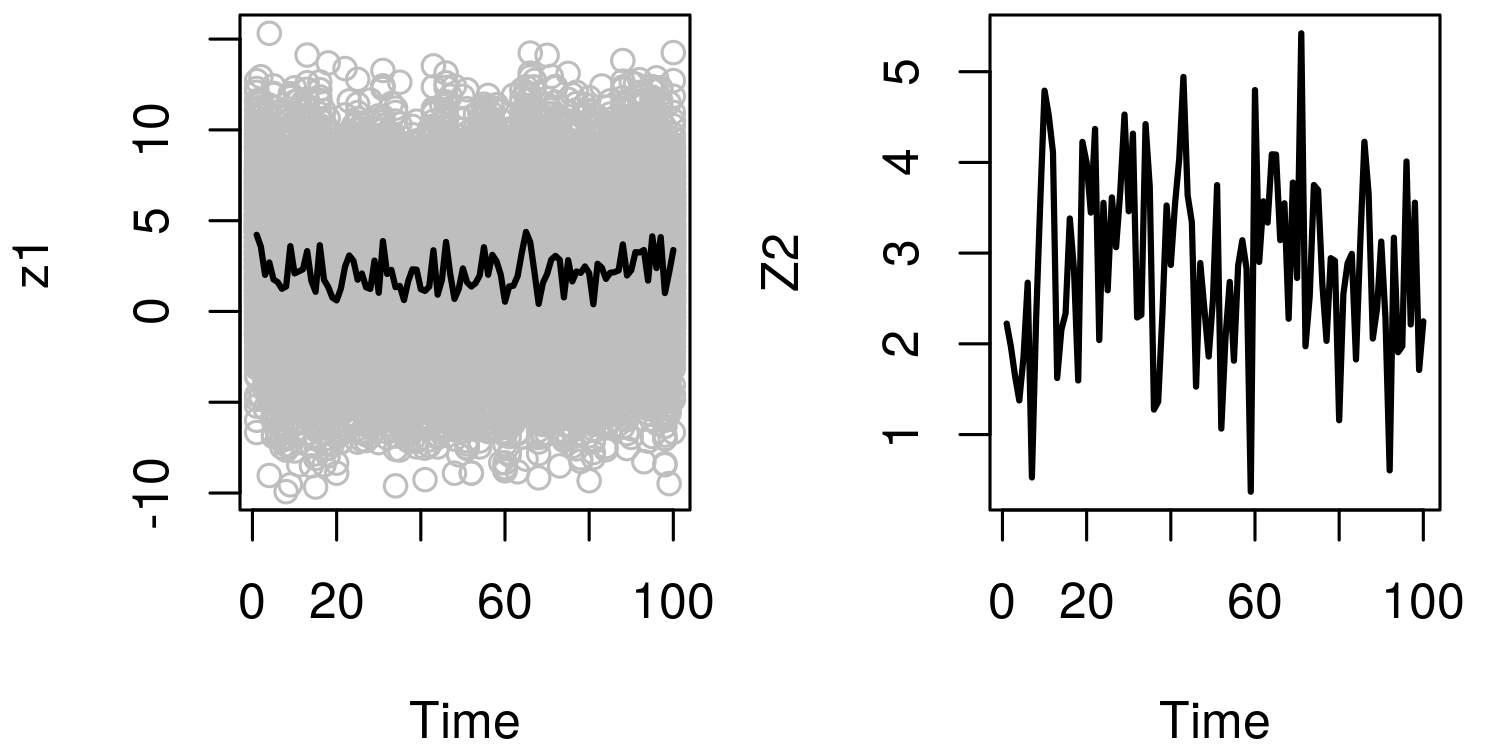
\includegraphics[width=\maxwidth]{figure/f-1} 

\end{knitrout}
\end{figure}
\end{frame}

\section{Model Estimation}
\subsection{}
\begin{frame}[fragile]%[allowframbreaks]
\frametitle{Results without ArfimaMLM I}
\begin{knitrout}
\definecolor{shadecolor}{rgb}{0.969, 0.969, 0.969}\color{fgcolor}\begin{kframe}
\begin{alltt}
\hlstd{m1a} \hlkwb{<-} \hlkwd{lm}\hlstd{(y} \hlopt{~} \hlstd{x1} \hlopt{+} \hlstd{x2} \hlopt{+} \hlstd{z1} \hlopt{+} \hlstd{z2,} \hlkwc{data} \hlstd{= data)}

\hlstd{m1b} \hlkwb{<-} \hlkwd{lmer}\hlstd{(y} \hlopt{~} \hlstd{x1} \hlopt{+} \hlstd{x2} \hlopt{+} \hlstd{z1} \hlopt{+} \hlstd{z2}
            \hlopt{+} \hlstd{(}\hlnum{1} \hlopt{|} \hlstd{time),} \hlkwc{data} \hlstd{= data)}

\hlstd{m1c} \hlkwb{<-} \hlkwd{lmer}\hlstd{(y} \hlopt{~} \hlstd{x1} \hlopt{+} \hlstd{x2} \hlopt{+} \hlstd{z1} \hlopt{+} \hlstd{z2}
            \hlopt{+} \hlstd{(}\hlnum{1} \hlopt{+} \hlstd{x1} \hlopt{|} \hlstd{time),} \hlkwc{data} \hlstd{= data)}
\end{alltt}
\end{kframe}
\end{knitrout}
\end{frame}

\subsection{}
\begin{frame}[fragile]\tiny%[allowframbreaks]
\frametitle{Results without ArfimaMLM II}

% Table created by stargazer v.5.2 by Marek Hlavac, Harvard University. E-mail: hlavac at fas.harvard.edu
% Date and time: Wed, Nov 18, 2015 - 02:41:53 PM
% Requires LaTeX packages: dcolumn 
\begin{table}[!htbp] \centering 
  \caption{Results for Simple OLS and Multilevel Model} 
  \label{ols_mle} 
\begin{tabular}{@{\extracolsep{5pt}}lD{.}{.}{-3} D{.}{.}{-3} D{.}{.}{-3} } 
\\[-1.8ex]\hline 
\hline \\[-1.8ex] 
 & \multicolumn{3}{c}{\textit{Dependent variable:}} \\ 
\cline{2-4} 
\\[-1.8ex] & \multicolumn{3}{c}{y} \\ 
\\[-1.8ex] & \multicolumn{1}{c}{\textit{OLS}} & \multicolumn{2}{c}{\textit{linear}} \\ 
 & \multicolumn{1}{c}{\textit{}} & \multicolumn{2}{c}{\textit{mixed-effects}} \\ 
\\[-1.8ex] & \multicolumn{1}{c}{(1)} & \multicolumn{1}{c}{(2)} & \multicolumn{1}{c}{(3)}\\ 
\hline \\[-1.8ex] 
 x1 & 0.200^{***} & 0.207^{***} & 0.207^{***} \\ 
  & (0.003) & (0.002) & (0.011) \\ 
  x2 & -0.050^{***} & -0.050^{***} & -0.050^{***} \\ 
  & (0.0002) & (0.0001) & (0.0001) \\ 
  z1 & 0.025^{***} & 0.003^{*} & 0.003^{*} \\ 
  & (0.002) & (0.002) & (0.001) \\ 
  z2 & -0.223^{***} & -0.224^{**} & -0.181^{*} \\ 
  & (0.006) & (0.106) & (0.099) \\ 
  Constant & 11.546^{***} & 11.567^{***} & 11.455^{***} \\ 
  & (0.024) & (0.325) & (0.304) \\ 
 \hline \\[-1.8ex] 
Observations & \multicolumn{1}{c}{50,000} & \multicolumn{1}{c}{50,000} & \multicolumn{1}{c}{50,000} \\ 
R$^{2}$ & \multicolumn{1}{c}{0.655} &  &  \\ 
Log Likelihood &  & \multicolumn{1}{c}{-72,501.370} & \multicolumn{1}{c}{-71,566.660} \\ 
Bayesian Inf. Crit. &  & \multicolumn{1}{c}{145,078.500} & \multicolumn{1}{c}{143,230.700} \\ 
\hline 
\hline \\[-1.8ex] 
\textit{Note:}  & \multicolumn{3}{r}{$^{*}$p$<$0.1; $^{**}$p$<$0.05; $^{***}$p$<$0.01} \\ 
\end{tabular} 
\end{table} 

\end{frame}

\subsection{}
\begin{frame}[fragile]%[allowframbreaks]
\frametitle{Results using ArfimaMLM I}
\begin{knitrout}
\definecolor{shadecolor}{rgb}{0.969, 0.969, 0.969}\color{fgcolor}\begin{kframe}
\begin{alltt}
\hlstd{m2a} \hlkwb{<-} \hlkwd{arfimaMLM}\hlstd{(y.ydif} \hlopt{~} \hlstd{x1.xdif} \hlopt{+} \hlstd{x2} \hlopt{+} \hlstd{z1.fd} \hlopt{+} \hlstd{z2.fd}
                \hlopt{+} \hlstd{(}\hlnum{1} \hlopt{|} \hlstd{time)}
                \hlstd{,} \hlkwc{data} \hlstd{= data,} \hlkwc{timevar} \hlstd{=} \hlstr{"time"}\hlstd{)}

\hlstd{m2b} \hlkwb{<-} \hlkwd{arfimaMLM}\hlstd{(y.ydif} \hlopt{~} \hlstd{x1.xdif} \hlopt{+} \hlstd{x2} \hlopt{+} \hlstd{z1.fd} \hlopt{+} \hlstd{z2.fd}
                 \hlopt{+} \hlstd{(}\hlnum{1} \hlopt{+} \hlstd{x1.xdif} \hlopt{|} \hlstd{time)}
                \hlstd{,} \hlkwc{data} \hlstd{= data,} \hlkwc{timevar} \hlstd{=} \hlstr{"time"}\hlstd{)}
\end{alltt}
\end{kframe}
\end{knitrout}
\end{frame}

\subsection{}
\begin{frame}[fragile]\tiny%[allowframbreaks]
\frametitle{Results using ArfimaMLM II}

% Table created by stargazer v.5.2 by Marek Hlavac, Harvard University. E-mail: hlavac at fas.harvard.edu
% Date and time: Wed, Nov 18, 2015 - 02:41:57 PM
% Requires LaTeX packages: dcolumn 
\begin{table}[!htbp] \centering 
  \caption{Results for ArfimaMLM} 
  \label{arfimamlm} 
\begin{tabular}{@{\extracolsep{5pt}}lD{.}{.}{-3} D{.}{.}{-3} } 
\\[-1.8ex]\hline 
\hline \\[-1.8ex] 
 & \multicolumn{2}{c}{\textit{Dependent variable:}} \\ 
\cline{2-3} 
\\[-1.8ex] & \multicolumn{2}{c}{y.ydif} \\ 
\\[-1.8ex] & \multicolumn{1}{c}{(1)} & \multicolumn{1}{c}{(2)}\\ 
\hline \\[-1.8ex] 
 x1.xdif & 0.203^{***} & 0.204^{***} \\ 
  & (0.002) & (0.011) \\ 
  x2 & -0.050^{***} & -0.050^{***} \\ 
  & (0.0001) & (0.0001) \\ 
  z1.fd & 0.204^{*} & 0.233^{**} \\ 
  & (0.118) & (0.105) \\ 
  z2.fd & -0.071 & -0.034 \\ 
  & (0.107) & (0.095) \\ 
  Constant & 0.055 & 0.055 \\ 
  & (0.110) & (0.110) \\ 
 \hline \\[-1.8ex] 
Observations & \multicolumn{1}{c}{47,500} & \multicolumn{1}{c}{47,500} \\ 
Log Likelihood & \multicolumn{1}{c}{-69,004.340} & \multicolumn{1}{c}{-68,091.650} \\ 
Akaike Inf. Crit. & \multicolumn{1}{c}{138,022.700} & \multicolumn{1}{c}{136,201.300} \\ 
Bayesian Inf. Crit. & \multicolumn{1}{c}{138,084.100} & \multicolumn{1}{c}{136,280.200} \\ 
\hline 
\hline \\[-1.8ex] 
\textit{Note:}  & \multicolumn{2}{r}{$^{*}$p$<$0.1; $^{**}$p$<$0.05; $^{***}$p$<$0.01} \\ 
\end{tabular} 
\end{table} 

\end{frame}

\subsection{}
\begin{frame}
\frametitle{Getting the Package}
\begin{itemize}
\item on CRAN: \url{http://cran.r-project.org/web/packages/ArfimaMLM/}
\item on GitHub (development version): \url{https://github.com/pwkraft/ArfimaMLM/}
\end{itemize}
\end{frame}

 \begin{frame}
   \frametitle{References}
   \def\newblock{\hskip .11em plus .33em minus .07em}
   %\nocite{*}
 %  \begin{tiny}
   \bibliographystyle{/data/Copy/1-src/lit/apsr}
   \bibliography{/data/Copy/1-src/lit/Literature}
 %  \end{tiny}
 \end{frame}

\end{document}
